\section{Methods for prediction and analysis of roll damping}
\label{se:methods_for_prediction_and_analysis}

\subsection{Hydrodynamics}
\label{se:hydrodynamics}
The roll damping consists of linear and nonlinear components. At zero speed the nonlinear damping is caused by the two-dimensional separation at the bilge keel or near the bilge circle (Eddy damping $B_E$). While at speed the nonlinear damping is mainly caused by the hydrodynamic lift force on the hull, represented as lift damping $B_L$. $B_E$ vanishes at high speed ($F_n>0.15)$ \cite{ikeda_components_1978}.

The wave damping also changes at speed. Ikeda \cite{ikeda_components_1978} proposes a formula for the fraction between wave damping at speed and zero speed: $\frac{B_W}{B_{W0}}$

The Ikeda method has been used to calculate the roll damping for a PCTC vessel Faust \cite{soder_assessment_2019}.
\begin{figure}[h]
    \centering
    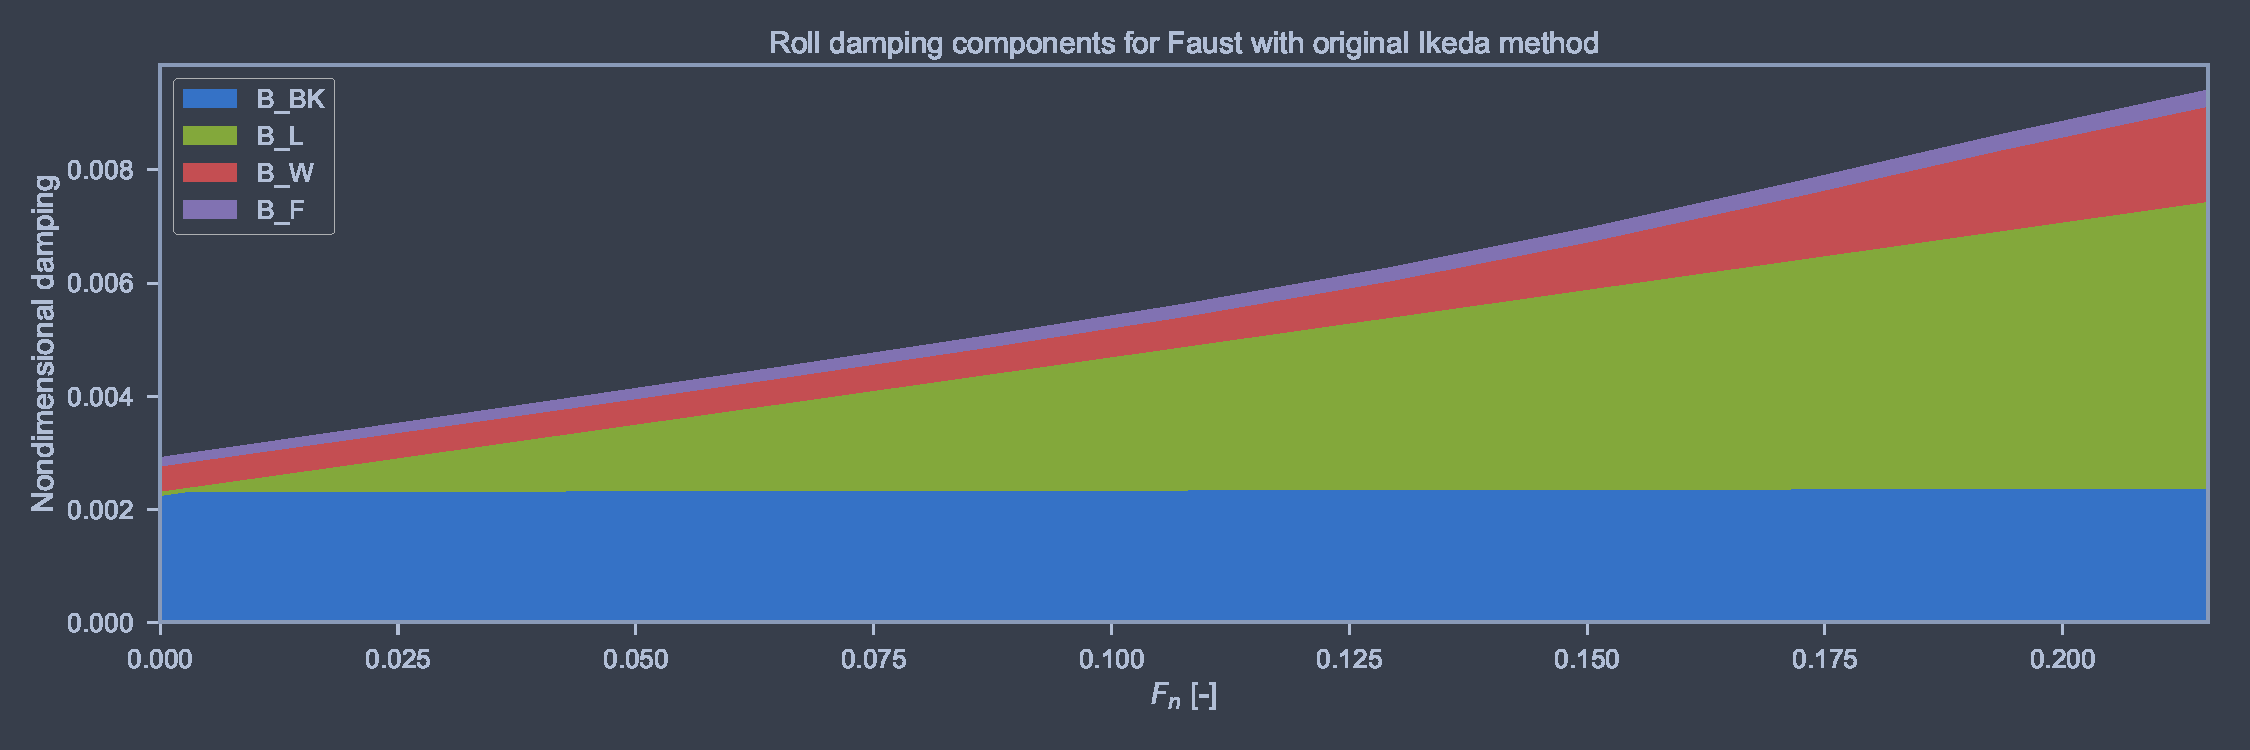
\includegraphics[width=\columnwidth]{figures/ikeda_faust.pdf}
    \caption{Roll damping components calculated with Ikeda method for PCTC Faust}
    \label{fig:ikeda_faust}
\end{figure}

\subsection{Existing semi-empirical methods}
\cite{ikeda_eddy_1978}, \cite{ikeda_roll_1979}, \cite{ikeda_components_1978}
Ikedas original method require strip method calculations. This is not an attractive option for the present study since that would require calculations with exact hull geometries to be carried out for all of the ships in the study. There exist however a \emph{Simplified Ikeda method} \cite{kawahara_simple_2011} that is instead used in this study \emph{Simplified Ikeda method} predicts the roll damping components at zero speed.

A study of the has been conducted which shows the roll damping components for various speeds. Calculations with *Ikeda original method* and the *Simplified method* have been carried for two ships (*S175* and *Faust*). The two methods show reasonable agreement for zero speed.

In order to introduce a speed dependency to the *Simplified method* the following is conducted:
* Add Lift damping $B_L$.
* Add speed dependence of wave damping $\frac{B_W}{B_{W0}}$
* Remove $B_E$ at ($F_n>0.15$) ?

\subsection{Equations}
\label{se:equations}
The roll motion can be written as \cite{himeno_prediction_1981}:
\begin{equation} \label{eq:roll_equation_himeno}
A_{44} \ddot{\phi} + \operatorname{B_{44}}\left(\dot{\phi}\right) + \operatorname{C_{44}}\left(\phi\right) = \operatorname{M_{44}}\left(\omega t\right)
\end{equation}


The equation express the roll moment [Nm] along a longitudinal axis though the centre of gravity.
Where $A_{44}$ is the virtual mass moment of inertia, $B_{44}$ is the roll damping moment and $C_{44}$ is the restoring moment. $M_{44}$ represents the external moment (usually moment from external waves).

The roll damping moment $B_{44}$ is the primary interest in this paper. The $B_{44}$ is determined using model scale roll decay tests. $B_{44}$ is determined using system identification, by finding the best fit to the following equation:
\begin{equation} \label{eq:roll_decay_equation_general_himeno}
A_{44} \ddot{\phi} + \operatorname{B_{44}}\left(\dot{\phi}\right) + \operatorname{C_{44}}\phi = 0
\end{equation}

The external moment is zero during a roll decay test, since there are no external forces present.

The $B_{44}$ can be expressed as a series expansion:  
$ B_{44} = B_1\cdot\dot{\phi} + B_2\cdot\dot{\phi}\left|\dot{\phi}\right| + B_3\cdot\dot{\phi}^3 + ...$

Truncating this series at the cubic term gives a "cubic model":
\begin{equation}
A_{44} \ddot{\phi} + \left(B_{1} + B_{2} \left|{\dot{\phi}}\right| + B_{3} \dot{\phi}^{2}\right) \dot{\phi} + \left(C_{1} + C_{3} \left|{\phi}\right| + C_{5} \phi^{2}\right) \phi = 0
\end{equation}


Truncating this series at the quadratic term gives a "quadratic model":Truncating this series at the quadratic term gives a "quadratic model":
\begin{equation} \label{eq:roll_decay_equation_himeno_quadratic}
A_{44} \ddot{\phi} + \left(B_{1} + B_{2} \left|{\dot{\phi}}\right|\right) \dot{\phi} + \operatorname{C_{2}} \phi = 0
\end{equation}


Truncating this series at the linear term gives a "linear model":
\begin{equation}
A_{44} \ddot{\phi} + B_{1} \dot{\phi} + \operatorname{C_{44}}\left(\phi\right) = 0
\end{equation}


Peter Piehl \cite{henry_peter_piehl_ship_nodate} shows an analytical solution to the linear model in equation \ref{eq:roll_decay_equation_himeno_linear}, where the natural frequency of the motion is obtained by:
\begin{equation}
\omega_{0} = \sqrt{\frac{C}{A_{44}}}
\end{equation}


The roll damping and the natural frequency can be made non dimensional using the following expressions \cite{himeno_prediction_1981}: 
\begin{equation} \label{eq:B44_hat_equation}
B_{44 hat} = \frac{\sqrt{2} \sqrt{\frac{beam}{g}} \operatorname{B_{44}}\left(\dot{\phi}\right)}{2 Disp beam^{2} \rho}
\end{equation}

\begin{equation} \label{eq:omega_hat_equation}
\omega_{hat} = \frac{\sqrt{2} \omega \sqrt{\frac{beam}{g}}}{2}
\end{equation}


\subsection{Analytical solution}
\label{se:analytical_solution}
\subsection{System identification}
\label{se:system_identification}
In order to extract roll damping parameters from the roll decay tests, parameters in the cubic, quadratic or linear roll decay models should be identified. The roll angle is measured during the roll decay tests. The system identification is defined as finding the parameters that produce a simulated roll signal that best fits the roll decay test measurement. The goodness of the fit is described using the coefficient of determination:
\begin{equation} \label{eq:R2}
R^2=1-\frac{SS_{res}}{SS_{tot}}
\end{equation}
Where $SS_{res}$ is sum of squares of residuals and $SS_{tot}$ is total sum of squares.

The parameters are found by solving a nonlinear least-squares problem using the Trust Region Reflective algorithm with smooth approximation of l1 (absolute value) loss which is usually a good choice for robust least squares.